\documentclass[10pt, xcolor={dvipsnames}]{beamer}
\mode<presentation>{
  \usetheme{Madrid}
  % or ...
  %\usecolortheme[named=OliveGreen]{structure}
  \setbeamercovered{transparent}
  % or whatever (possibly just delete it)
}
\usepackage[utf8x]{inputenc}
\usepackage[russian]{babel}
\usepackage[usenames,dvipsnames]{pstricks}
\usepackage{epsfig}
\begin{document}
\small
\begin{frame}{Триангуляция Делоне, Триангуляция -> Граф}
\begin{itemize}
\item Берется структура в PDB.
\item Центры атомов рассматриваются как точки. По ним строится триангуляция Делоне (с помощью scipy.delaunay - обертки над алгоритмом qhull).
\item Берется не взвешенная триангуляция -- по тем же соображениям, по которым она используется в CAVER (эвристика).
\end{itemize}
Я сопоставляю графу триангуляцию по тому же принципу, как в статье по CAVER:
\begin{columns}
\begin{column}{0.5\textwidth}
\begin{center}
\resizebox{!}{0.3\textheight}{
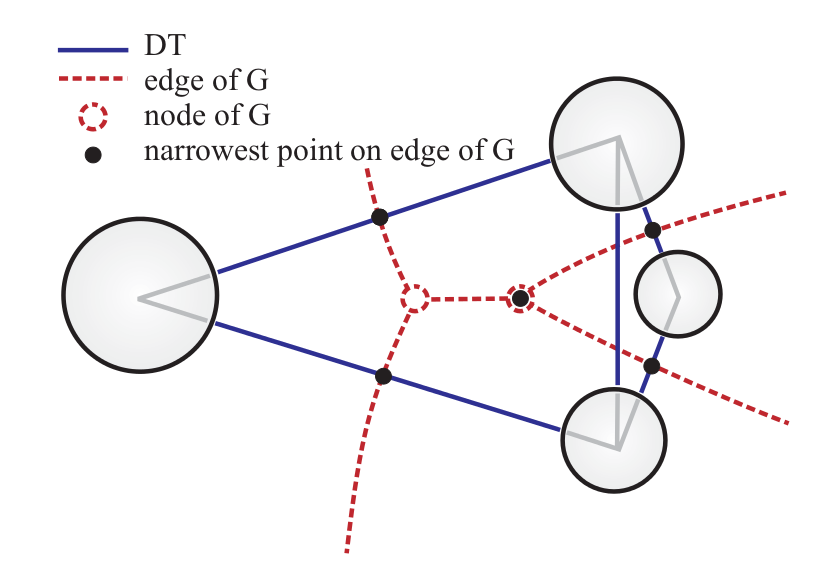
\includegraphics{image4_caver.png}
}

[Computation of tunnels in protein molecules using
Delaunay triangulation, P.Medek, et al., 2007]
\end{center}
\end{column}
\begin{column}{0.5\textwidth}
Треугольники триангуляции -- вершины графа, ребра графа -- общие стороны треугольников (с ограничением снизу на длину).

Дополнительно используется такой же граф по треугольникам выпуклой оболочки (без ограничения снизу на длину стороны, просто по смежным по стороне треугольникам).
\end{column}
\end{columns}


\end{frame}

\begin{frame}{Алгоритм (шаг 1)}
Выбирается начальное множество треугольников выпуклой оболочки. Например, берутся треугольники, вершины которых недалеко (в смысле отсечки по расстоянию) от второго белка.

Дополнительно могут быть усложнения.

\begin{itemize}
\item В CAVER используется алгоритм Дейкстры для поиска каналов максимальной ширины. Каналы как правило сквозные, в нашем случае это не обязательно.
\item Нам надо получить внешнюю поверхность белка, то есть все, что расположено близко к интерфейсу взаимодействия, и при этом может быть, например, карманом (углублением в поверхности) или каналом (сквозной дырой в поверхности).
\end{itemize}
\end{frame}

\begin{frame}{Алгоритм (шаг 2 -- основной) }{мотивация использовать Дейкстру в каком-то виде}
\begin{itemize}
\item Попробуем искать карманы. Для этого используем поиск в ширину с ограничением на проходимость ребер. 
\item Вот что получается (след слайд - выделяются много-много атомов по всей внешней поверхности белка):
\end{itemize}
\begin{center}
\resizebox{!}{0.5\textheight}{
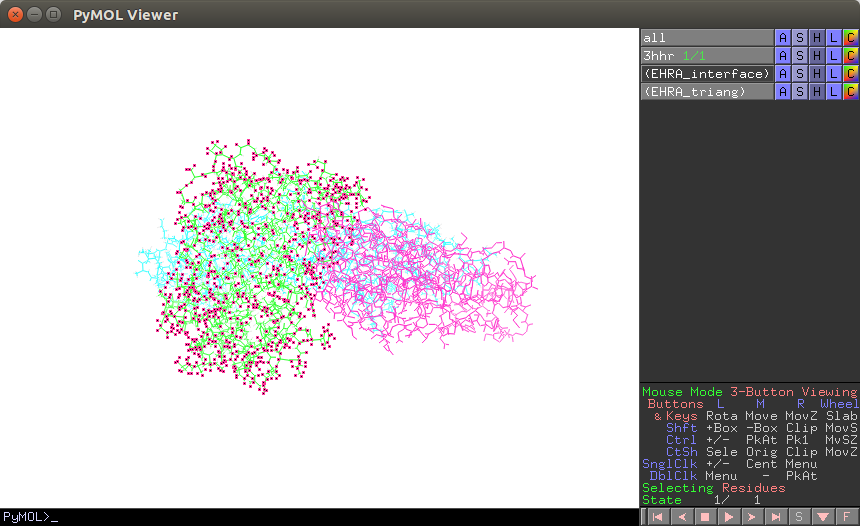
\includegraphics{dijkstra1.png}
}
\end{center}
\end{frame}
\begin{frame}{Алгоритм (урезанный алгоритм Дейкстры)}{пока одни вопросы}
\begin{columns}
\begin{column}{0.3\textwidth}
\begin{center}
\resizebox{!}{0.2\textheight}{
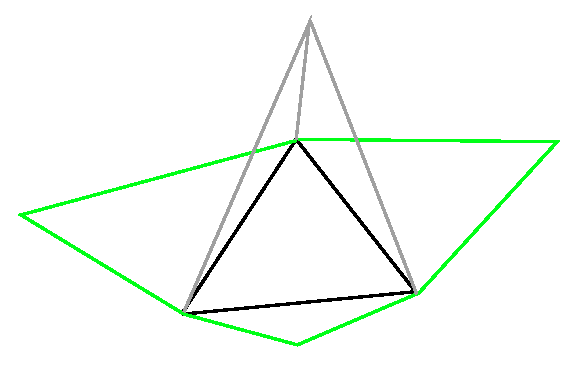
\includegraphics{triangles.eps}
}
\end{center}
\end{column}
\begin{column}{0.7\textwidth}
\small{
Идеи
\begin{itemize}
\item Начинаем с множества отобранных треугольников на шаге 1 и их соседей (выделены зеленым на рисунке).
\item неясен принцип, по которому лучше присваивать метки треугольникам. То есть на первом этапе понятно, метка 0 присваивается треугольникам выпуклой оболочки. На следующих - хз
\item Понятно, как ограничить поиск -- ходить только по тем треугольникам, для которых ближайший треугольник выпуклой оболочки -- один из отобранных, а не их соседей.
 Но надо понять, в каком смысле ближайший
\end{itemize}
}
\end{column}
\end{columns}

\end{frame}

\begin{frame}{Алгоритм (шаг 2 -- основной) }{что есть}
\begin{itemize}
\item Нечто из космоса:
\end{itemize}
\begin{center}
\resizebox{!}{0.8\textheight}{
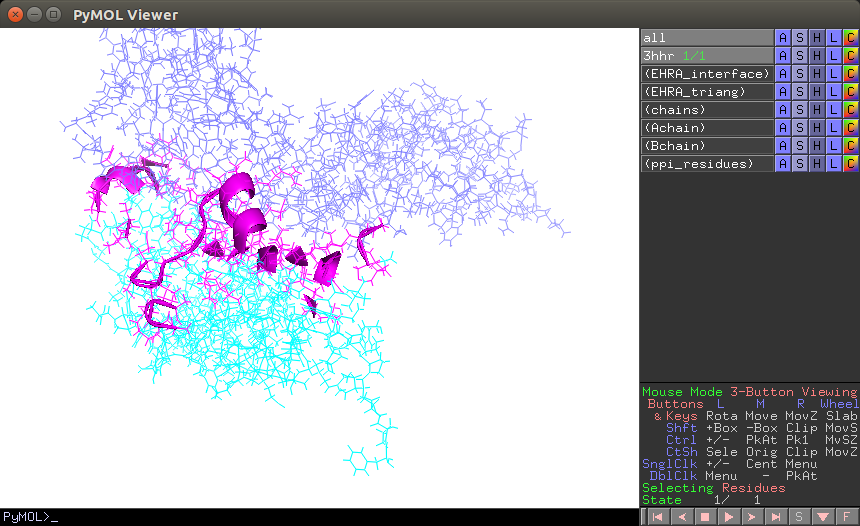
\includegraphics{image_step2.png}
}
\end{center}
\end{frame}

\end{document}